\begin{Schunk}
\begin{Sinput}
> library("Ham94", lib.loc = "../../../library")
\end{Sinput}
\end{Schunk}
Page 697 describes an example of the application of Markov switching models to US GNP from 1951Q1 to 1984Q4.
\begin{Schunk}
\begin{Sinput}
> data(gnpdata, package = "Ham94")
> selection <- subset(gnpdata, Quarter >= "1951-01-01" & Quarter <= 
+     "1984-04-01")
> d <- selection$Quarter[-1]
> g <- diff(100 * log(selection$GNP), lag = 1, differences = 1)
\end{Sinput}
\end{Schunk}

The actual implementation uses the technique of collapsing multi-period states into a single state, p691, p698.
During the maximum likelihood estimation process the state probabilities will change, but the layout of the matrix
is still the same.  The following code fragment precalculates the transition matrix structure with the five possible
values, then uses a separate 5 element lookup vector to populate it.
\begin{Schunk}
\begin{Sinput}
> nlags <- 4
> nstates <- 2^(nlags + 1)
> lagstate <- 1 + outer(1:nstates, 1:(nlags + 1), FUN = function(i, 
+     j) {
+     trunc((i - 1)/2^(nlags + 1 - j))%%2
+ })
> transit <- outer(X = 1:nstates, Y = 1:nstates, FUN = function(i, 
+     j) {
+     ((2 * lagstate[i, 1] + lagstate[j, 1] - 1) - 1) * (((i - 
+         1)%%(2^nlags)) == trunc((j - 1)/2)) + 1
+ })
\end{Sinput}
\end{Schunk}
The bulk of the work is done by the following function, based on the algorithm in section 22.4.
Ergodic probabilities are defined as on page 684, including equation [22.2.26].
The loop uses equations [22.4.24], [22.4.2], [22.4.5], [22.4.8], [22.4.7], [22.4.6] and [22.4.14].
\begin{Schunk}
\begin{Sinput}
> infer.regimes <- function(THETA, YT) {
+     phi <- THETA[grep("phi*", names(THETA))]
+     mu <- THETA[grep("mu*", names(THETA))]
+     sigma <- THETA["sigma"]
+     p11star <- THETA["p11star"]
+     p22star <- THETA["p22star"]
+     T <- length(YT)
+     tp <- c(0, p11star, 1 - p22star, 1 - p11star, p22star)
+     P <- array(tp[transit], c(nstates, nstates))
+     A <- rbind(diag(nstates) - P, rep(1, nstates))
+     ergodic.pi <- (solve(t(A) %*% A) %*% t(A))[, nstates + 1]
+     xi.t.t <- ergodic.pi %o% rep(1, nlags)
+     xi.t.t_1 <- cbind(xi.t.t, ergodic.pi)
+     log.likelihood <- 0
+     for (tt in (nlags + 1):T) {
+         residuals <- as.vector(((rep(1, nstates) %o% YT[tt:(tt - 
+             nlags)]) - array(mu[lagstate], c(nstates, nlags + 
+             1))) %*% c(1, -phi))
+         eta.t <- dnorm(residuals, mean = 0, sd = sigma)
+         fp <- eta.t * xi.t.t_1[, tt - 1]
+         fpt <- sum(fp)
+         xi.t.t <- cbind(xi.t.t, fp/fpt)
+         log.likelihood <- log.likelihood + log(fpt)
+         xi.t.t_1 <- cbind(xi.t.t_1, P %*% xi.t.t[, tt])
+     }
+     xi.t.T <- xi.t.t[, T] %o% 1
+     for (tt in (T - 1):1) xi.t.T <- cbind(xi.t.t[, tt] * (t(P) %*% 
+         (xi.t.T[, 1]/xi.t.t_1[, tt + 1])), xi.t.T)
+     list(log.likelihood = log.likelihood, xi.t.t = xi.t.t, xi.t.T = xi.t.T)
+ }
\end{Sinput}
\end{Schunk}
Initial values of the parameters for transition probabilities are set from historical averages.
The phi and sigma values are obtained from a (non-state) regression of change in GDP on 4 of its own lags.
\begin{Schunk}
\begin{Sinput}
> g.lm <- lm(g ~ 1 + g_lag, list(g = g[-1:-nlags], g_lag = embed(g[-length(g)], 
+     nlags)))
> THETA <- c(p11star = 0.85, p22star = 0.7, mu = c(1, 0), phi = as.vector(g.lm$coefficients[1 + 
+     (1:nlags)]), sigma = summary(g.lm)$sigma)
\end{Sinput}
\end{Schunk}
Now we are in a position to optimize, then calculated the smoothed probabilities from the
optimal parameters. 
\begin{Schunk}
\begin{Sinput}
> objective <- function(THETA, YT) {
+     -infer.regimes(THETA, YT)$log.likelihood
+ }
> optimizer.results <- optim(par = THETA, hessian = TRUE, fn = objective, 
+     gr = NULL, YT = g)
> se <- diag(solve(optimizer.results$hessian))^0.5
> print(optimizer.results$par)
\end{Sinput}
\begin{Soutput}
     p11star      p22star          mu1          mu2         phi1         phi2 
 0.869651020  0.657920015  1.095327317 -0.198544833  0.311107386  0.092829514 
        phi3         phi4        sigma 
-0.125038400 -0.007166502  0.872625052 
\end{Soutput}
\begin{Sinput}
> print(se)
\end{Sinput}
\begin{Soutput}
   p11star    p22star        mu1        mu2       phi1       phi2       phi3 
0.13323951 0.04404274 0.23169921        NaN 0.08762475 0.10748667 0.09374541 
      phi4      sigma 
0.08826466        NaN 
\end{Soutput}
\begin{Sinput}
> regimes <- infer.regimes(optimizer.results$par, g)
> recession.probability <- as.vector((1:nstates > nstates/2) %*% 
+     regimes$xi.t.t)
> smoothed.recession.probability <- as.vector((1:nstates > nstates/2) %*% 
+     regimes$xi.t.T)
\end{Sinput}
\end{Schunk}
The results are shown below.
\begin{center}
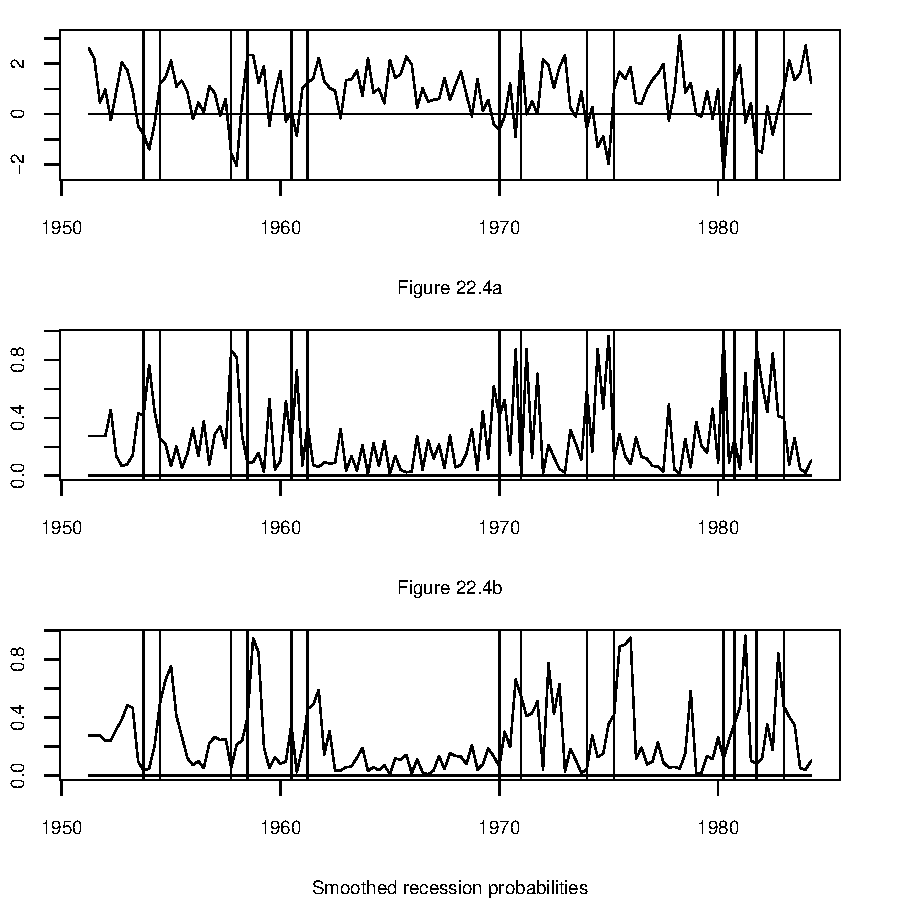
\includegraphics{p697-007}
\end{center}
